\documentclass{standalone}
\usepackage{tikz, graphicx, cmbright, amsmath, setspace}
\begin{document}
%\fontsize{10pt}{1em}\selectfont
\setstretch{0.9}


\begin{tikzpicture}[scale=0.75, every node/.style={scale=0.75}]
\node [above right] at (0, 0) {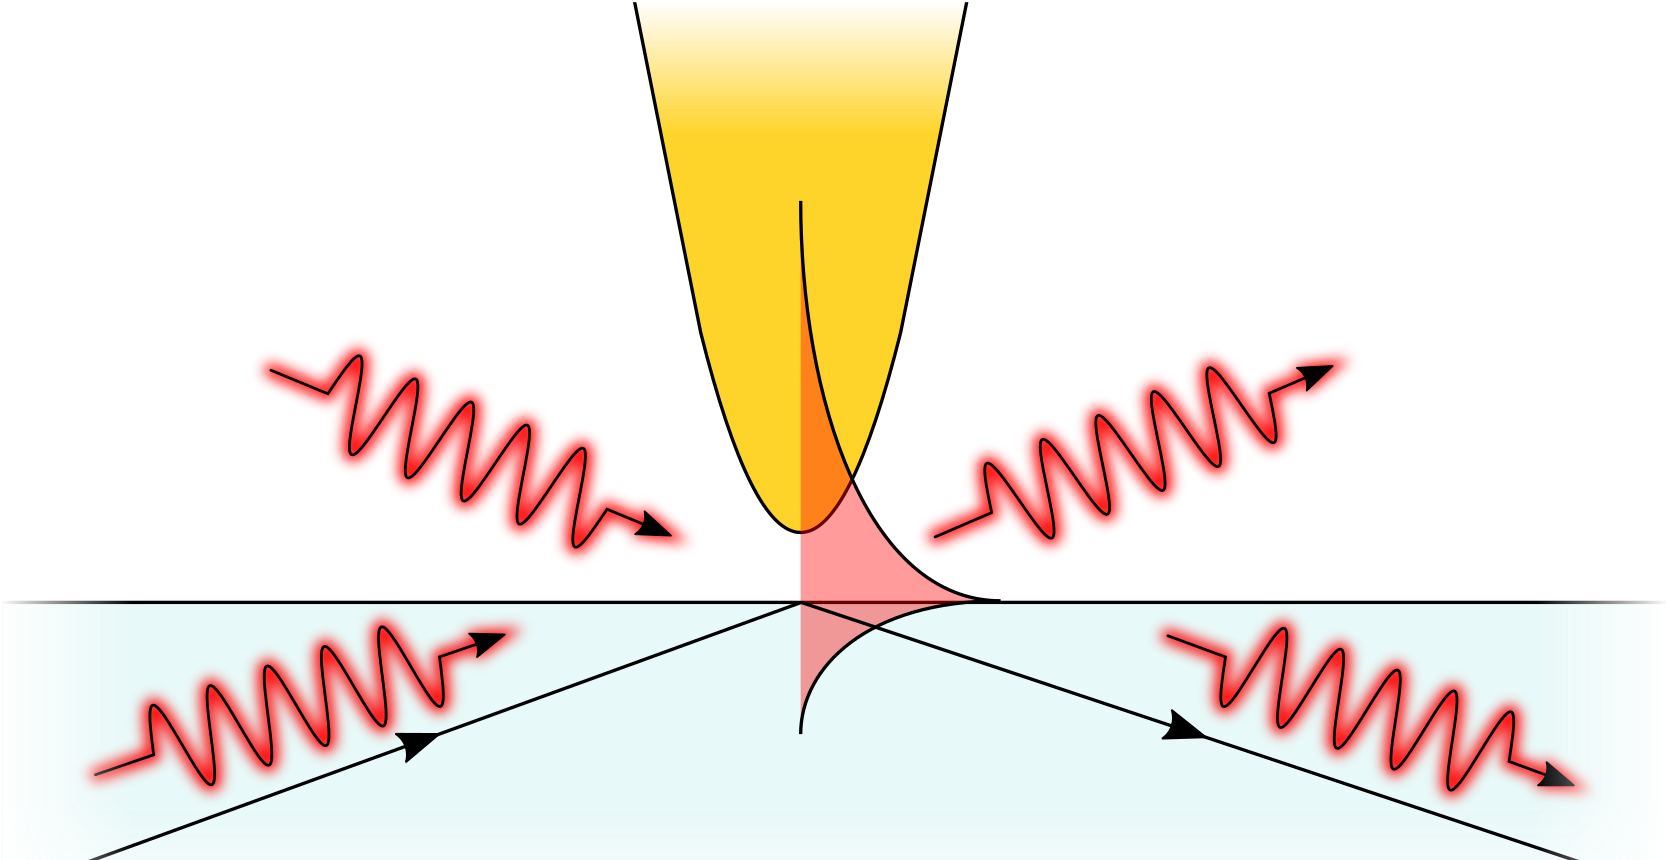
\includegraphics[width=9cm]{tenom_basic.png}};
\node at (-0.8,4.8) {(a)};

\draw (-0.8,1.8) circle (0.25);
\node at (-0.8,1.8) {1};
\node [align=center] at (4.4,0.45) {evanescent wave\\generation};
\node [align=center] at (0,1.1) {TIR excitation\\$\mathit{NA}>1$};


\draw (0.95,3.1) circle (0.25);
\node at (0.95,3.1) {2};
\node at (1.4,2.9) {$\omega$};
%\node [left] at (10.8,4) {$\omega - \delta\omega$};
\node [left] at (10.8,2.9) {\bfseries$
\begin{cases}
    \omega & \text{a-SNOM}\\
    \omega - \delta\omega & \text{TERS}
\end{cases}
$};

\draw (7.8,3.8) circle (0.25);
\node at (7.8,3.8) {3};
\node [align=left] at (6.25,3.35) {near--far-field\\scattering};

\draw (9.5,1.8) circle (0.25);
\node at (9.5,1.8) {4};
\node [align=center] at (9.3,1.1) {radiative\\SPP decay};

{\fontsize{7pt}{1em}\selectfont \bfseries
\color{blue}
\node at (4.2,2.45) {$-$};
\node at (4.45,2.1) {$-$};
\node at (4.7,2.45) {$-$};
\color{red}
\node at (4.3,2.25) {$+$};
\node at (4.6,2.25) {$+$};
}

\end{tikzpicture}

\end{document}